\chapter{Outils informatiques et données utilisées}

Dans cette thèse, nous avons développé des méthodes basées sur les \gls{ia} pour exploiter les données multimodales de patients. Pour cela, nous avons utilisé un vaste panel de ressources biologiques, d'outils informatiques et de méthodes \gls{ia}. Dans ce chapitre, nous allons décrire l'ensemble des outils et ressources utilisés pour construire nos méthodes d'analyse.

\section{Données biomédicales de myopathies congénitales}
Pour développer ces méthodes, nous nous sommes basés sur des données d'imagerie et des comptes rendus de biopsie. La source de ces données est présentée ci-dessous.

\subsection{Comptes rendus de biopsie de l'institut de myologie de Paris}
La première source de données provient de l'institut de myologie de Paris. Grâce à une collaboration avec l'équipe du laboratoire d’histopathologie d'abord dirigé par Norma B. Romero puis Teresinha Evangelista, nous avons pu récupérer et utiliser 192 comptes rendus de biopsie musculaire de patients atteints de myopathies (congénitales, dystrophies ou autre), dont 138 spécifiquement atteint par des myopathies congénitales identifiées. Ces rapports sous format papier ont été scannés puis anonymisés d'abord avec un outil d'anonymisation que nous avons développé (présenté dans le chapitre 7), puis vérifiés à la main. La figure \ref{fig:compte-rendu-exemple} présente la structure d'un compte rendu anonymisé de biopsie typique présent dans le jeu de données. Il y a deux types de comptes rendus, ceux qui concernent les observations en microscopie photonique et ceux qui concernent les observations en microscopie électronique. Cependant, cette structure peut varier en fonction de l'année de production du compte rendu, certains sont totalement déstructurés.

\begin{figure}[!ht]
 \centering
 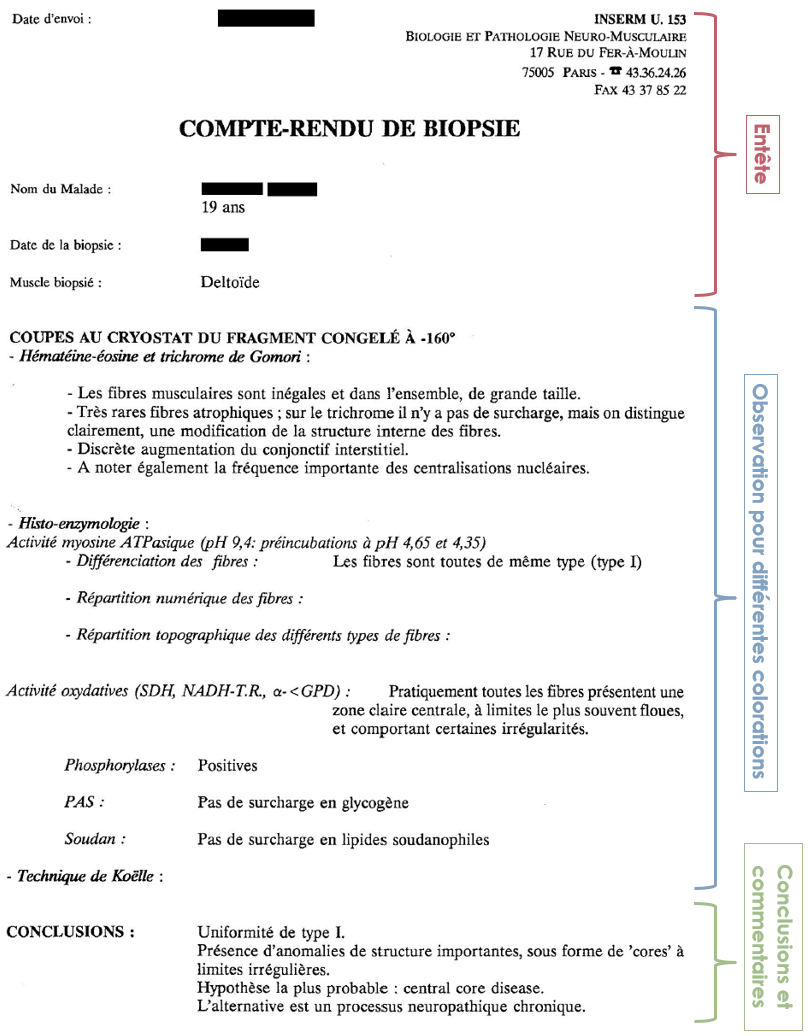
\includegraphics[width=0.9\textwidth]{figures/compte_rendu_exemple.png}
 \caption[Exemple de compte rendu de biopsie]{\textbf{Exemple de compte rendu de biopsie en microscopie photonique anonymisé de l'institut de myologie de Paris}. Les comptes rendus sont structurés en trois sections: une entête avec des informations générales sur la ptient, un corps de texte contenant une liste de colorations et les observations réalisée et une conclusion avec les diagnostic final et un commentaire optionel.}
 \label{fig:compte-rendu-exemple}
\end{figure}

\subsection{Images de biopsie musculaire de souris}
Une seconde source de données provient d'une collaboration avec l'\gls{igbmc}, plus spécifiquement avec l'équipe Physiopathologie des maladies neuromusculaires dirigée par Jocelyn Laporte. Cette équipe travaille sur les myopathies congénitales et utilise plusieurs souris modèles de myopathies congénitales. Ainsi en travaillant avec les membres de l'équipe réalisant des biopsies musculaires sur ces modèles, nous avons développé des méthodes d'analyse pour des biopsies musculaires de souris aux colorations \gls{he}, \gls{sdh}, ATPase et à fluorescence.

\section{Ontologies et nomeclatures en biologies}
En biologie, les ontologies sont des vocabulaires standards pour faciliter l'intégration des données et leur analyse. Dans cette thèse, pour standardiser les données issues des comptes rendus, notamment dans le cadre du développement de l'outil \gls{impatient} et l'analyse de sa base de données, nous avons utilisé diverses ontologies préexistantes que nous allons décrire ici.

\subsection{Ontologie des phénotypes : HPO}
L'ontologie \gls{hpo}, développée en 2008 par Peter N Robinson et Sebastian Köhler au \textit{Charité University Hospital} à Berlin (\cite{robinson_human_2008}, \cite{kohler_human_2021}), rassemble l'ensemble des phénotypes médicaux observables chez l'Homme. Organisée sous forme d'arbre, elle contient plus de 13 000 termes organisés selon un niveau croissant de précision (par exemple le terme "anomalie de l'œil" est un parent du terme "anomalie de la pupille"). Chaque terme est associé à un identifiant unique sous la forme HPO:XXXXX et possède un certain nombre d’annotations comme des maladies associées, des gènes associés, des synonymes, des publications associées. L'ensemble de ces informations est disponible en ligne sur le portail  \url{https://hpo.jax.org/} qui permet aussi de télécharger l'ontologie dans les formats standards (JSON, OBO, OWL). Cette ontologie est utilisée dans \gls{impatient} pour normaliser les observations cliniques des patients.

\subsection{Ontologie de maladies : ORDO par Orphanet}
L'\gls{ordo} est développée dans le cadre d'une collaboration entre Orphanet (\url{https://www.orpha.net/}, \cite{maiella_orphanet_2013}), et l'Institut Européen de Bioinformatique (EBI). Orphanet est une ressource informatique ayant pour but de répertorier l'ensemble des informations concernant les maladies rares et les médicaments orphelins. L'ontologie ORDO répertorie plus de 7 000 maladies rares connues. Chaque maladie rare est répertoriée sous un identifiant unique de la forme ORPHA:XXXXXX, par exemple la maladie "Myopathie congénitale sévère à némaline" correspond à l'identifiant ORPHA:171430. De plus, chaque maladie est associée à des annotations telles que leur prévalence, des synonymes, un mode d'hérédité, un âge d'apparition, un pronostic, les gènes causant la maladie et autre. Pour finir, chaque maladie est aussi liée à des symptômes cliniques grâce à un lien direct vers des identifiants de l'ontologie \gls{hpo}. Dans le cadre de notre outil \gls{impatient} nous avons utilisé cette ontologie pour normaliser le diagnostic final des patients.

\subsection{Nomenclature génétique : HGNC et HGVS}
La nomenclature HUGO (\url{https://www.genenames.org/}, acronyme de Human Genome Organisation, est gérée par le Comité de Nomenclature des Gènes de HUGO (HGNC) à l'Institut Européen de Bioinformatique. Ce comité est responsable de l'attribution de noms uniques pour les gènes humains, que ce soit des gènes codants pour des protéines, gènes non codants ou pseudogènes. Au total, plus de 43 000 noms de gènes uniques sont référencés et annotés avec des références croisées vers des bases de données externes (banque de séquences, orthologies, mutations, structures, Orphanet…). Concernant les variations génétiques (mutations), la nomenclature établie par la \gls{hgvs} (\url{https://www.hgvs.org/}) fait autorité. Cette nomenclature spécifie la façon de représenter textuellement un variant génétique. Par exemple selon cette nomenclature la notation "NM\_001164508.2(NEB):c.25336C>T (p.Arg8446Ter)" indique une mutation faux-sens dans la protéine NEB où l'acide aminé n° 8446 est substitué d'une arginine à un codon stop. La nomenclature HUGO et HGVS sont toutes deux intégrées dans \gls{impatient} (voir chapitre \ref{chap_imp}) pour codifier le diagnostic génétique des patients (gène muté et localisation de la mutation responsable de la maladie).

\section{Développement de modèles de ML traditionnels et xAI}
Dans le cadre de l'analyse de la base de données de \gls{impatient} et des résultats d'\textit{embedding} de \gls{nlmyo} nous avons utilisé des algorithmes de \gls{ml} traditionnels pour créer des modèles prédictifs. Dans cette section, nous présentons les principaux outils utilisés en ce qui concerne les algorithmes utilisés et l'analyse de leurs performances.

\subsection{\textit{Scikit-Learn} : une boite à outils pour l'apprentissage automatique}
\textit{Scikit-Learn} (version 1.3, \cite{pedregosa_scikit-learn_2011}, \url{https://scikit-learn.org/}) est une bibliothèque de code python mettant à disposition un grand nombre d'outils et permettant de préparer les données, d'entrainer des modèles de \textit{\gls{ml}} et d'évaluer ses performances. \textit{Scikit-learn} inclut des algorithmes de classification, de régression, de clustering, de réduction de dimensionnalité, d'optimisation et de sélection de modèles. Scikit-learn a été utilisé dans cette thèse pour : (i) partitionner et normaliser les données, (ii) entrainer des modèles de classification de différentes familles d'algorithmes, (iii) optimiser et évaluer les performances des modèles.

\subsection{Validation croisée et évaluation des performances}
La validation croisée (\textit{cross-validation }en anglais) est une technique d'évaluation de modèles prédictifs permettant d'avoir une estimation plus robuste et précise des métriques de performance. Cette méthode est particulièrement utile pour les jeux de données de petite taille. La figure \ref{fig:cross-val} présente schématiquement son fonctionnement. Le jeu de données initial est séparé en N sous-ensembles (nommés \textit{folds} ou bloc, ici au nombre de 5). Ensuite le modèle est entrainé sur l'ensemble des sous-ensembles à l'exception d’un, qui est utilisé comme jeu de test des performances. Ce processus est répété autant de fois qu'il y a de \textit{folds} afin que chaque \textit{fold} ait été utilisé exactement une fois comme jeu de test. Ainsi pour 5 \textit{folds}, cinq modèles sont entrainés et évalués. On peut alors calculer une performance moyenne du modèle entrainé sur l'ensemble des données, en calculant les performances moyennes des cinq modèles. Plus le nombre de \textit{folds} est important, plus cette moyenne est précise, mais c'est plus coûteux en temps et ressources de calcul, car il faut entrainer plus de modèles.
\begin{figure}[!ht]
 \centering
 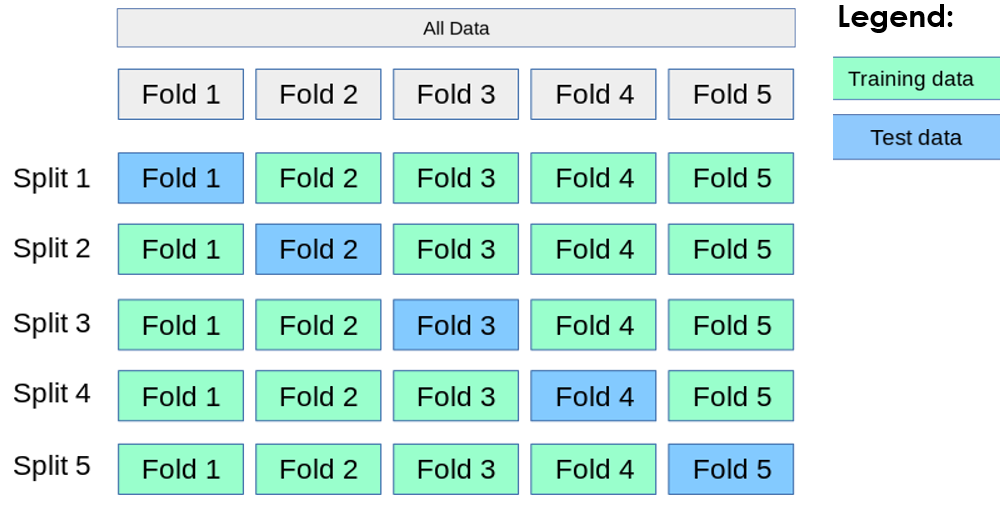
\includegraphics[width=0.9\textwidth]{figures/cross-val.png}
 \caption[Schéma validation-croisée]{\textbf{Schéma du principe de la validation croisée}. Ici la valiation-croisée est réalisée en \textit{5 folds}, chaque point de donné sera utilisé une fois dans le jeu de test et 4 fois dans 4 jeux d'entrainement (modifié de la documentation de \textit{Scikit-Learn}).}
 \label{fig:cross-val}
\end{figure}
\subsection{Recherche d'hyperparamètres}
La recherche d'hyperparamètres est une étape importante dans le développement de modèles prédictifs pour améliorer les performances des modèles. Les hyperparamètres sont des paramètres propres à chaque algorithme, qui sont spécifiés en amont de l'entrainement et qui ne varient pas lors de l'entrainement, mais qui influent directement sur les performances du modèle. Par exemple, dans le cadre de l'entrainement d'un arbre de décision, un exemple d'hyperparamètre peut être la profondeur maximale de l'arbre ou encore la méthode de calcul de qualité d'un nœud (par exemple méthode de gini ou entropie).
\begin{figure}[!ht]
 \centering
 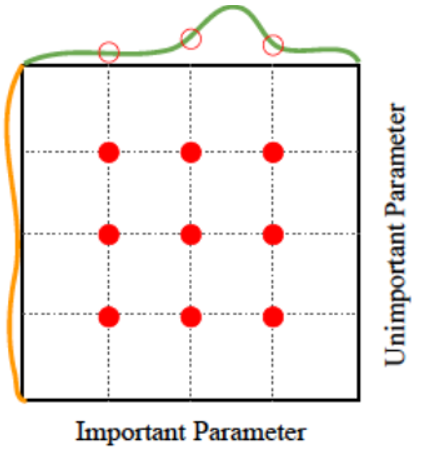
\includegraphics[width=0.3\textwidth]{figures/parameters_grid.png}
 \caption[Schéma rechercher hyper-paramètres]{\textbf{Schéma du principe de recherche d'hyperparamètres par grille pour 2 paramètres}. Un point rouge représente un modèle entrainé. Les courbes en abscisse et ordonnée représente les performances du modèle. Le paramètre en ordonnée n'a que très peu d'effet sur les performances, alors que les variations du paramètre en abscisse améliorent les performances du modèle.}
 \label{fig:params_grid}
\end{figure}
La recherche d'hyperparamètres revient à trouver une combinaison de paramètres optimale qui maximise les performances du modèle après entrainement. La méthode la plus classique pour cela est l'optimisation par grille. À partir d'un ensemble de valeurs possibles pour chaque paramètre, on va entrainer et tester les performances du modèle pour chaque combinaison de valeurs et sélectionner la combinaison de valeurs la plus performante. La figure \ref{fig:params_grid}  présente un exemple théorique d'optimisation par grille pour deux paramètres. Pour chacun des paramètres, 3 valeurs sont possibles, c'est donc un total de 9 modèles qui sont entrainés et testés. On peut alors mesurer l'impact de chaque paramètre sur les performances finales du modèle pour trouver le paramètre le plus important et sa valeur optimale.
D'autres méthodes moins naïves et moins coûteuses que la grille existent pour la recherche d'hyperparamètres telle que l'approche bayésienne utilisée par la bibliothèque de code \textit{Optuna} (\cite{akiba_optuna_2019},\url{https://optuna.org/}) qui permet de trouver une combinaison optimale plus rapidement.

\subsection{Algorithme de système de classeurs : ExSTraCS 2.0}
Les systèmes de classeurs sont une famille d'algorithmes de \gls{ml} considérés comme explicables. Dans cette thèse, nous avons utilisé le \gls{lcs} nommé \textit{ExSTraCS 2.0} (\cite{urbanowicz_exstracs_2015}), spécifiquement développé pour les tâches de classification à partir de données complexes, hétérogènes et de haute dimensionnalité. Cet algorithme a été utilisé pour tenter de prédire le diagnostic de sous-type de myopathies congénitales des patients à partir des annotations réalisées dans \gls{impatient}. L'implémentation en Python de cet algorithme de \gls{lcs} nommée \textit{scikit-ExSTraCS} (\url{https://github.com/UrbsLab/scikit-ExSTraCS}) nous a permis d'entrainer un modèle basé sur cette méthode et de comparer ses performances aux autres algorithmes implémentés dans \textit{scikit}, \textit{via} le \textit{pipeline} d'entrainement et de comparaison de modèles nommé \textit{Streamline}.

\subsection{Streamline: un \textit{pipeline} d'entrainement et de comparaison de modèles ML}
Pour entrainer le modèle de classification le plus performant possible dans le cadre de  l'analyse de la base de données d'\gls{impatient}, nous avons utilisé le \textit{pipeline} d'entrainement et de comparaison de modèles de \gls{ml} nommé \textit{Streamline} (\cite{urbanowicz_streamline_2023}). La figure \ref{fig:streamline} (\cite{urbanowicz_streamline_2023}) présente son fonctionnement. Il y a 4 étapes principales. L'étape 1 (modules 1 et 2) consiste en la lecture, exploration statistique et préparation des données. L'étape 2 (modules 3 et 4) consiste au calcul de l'importance de chaque annotation (comprendre ici : \textit{feature}) et en la sélection des annotations les plus pertinentes pour la classification. L'étape 3 (module 5) consiste à l'optimisation et l'entrainement de 16 algorithmes de \gls{ml} variés et l'évaluation des performances des modèles issus de cet entrainement. Finalement, l'étape 4 (modules 6, 7, 8  et 9) correspond à la phase de post-traitement, où seront générés les figures de comparaison des performances des modèles et le nettoyage des fichiers. STREAMLINE n'est pour l'instant disponible que pour faire de la classification binaire. Nous nous intéressons à un problème de classification multi-classe (prédiction de diagnostic), donc nous avons modifié le pipeline pour le rendre compatible avec nos données. Le code du pipeline modifié est accessible à l'adresse \url{https://github.com/lambda-science/STREAMLINE}.
\begin{figure}[!ht]
 \centering
 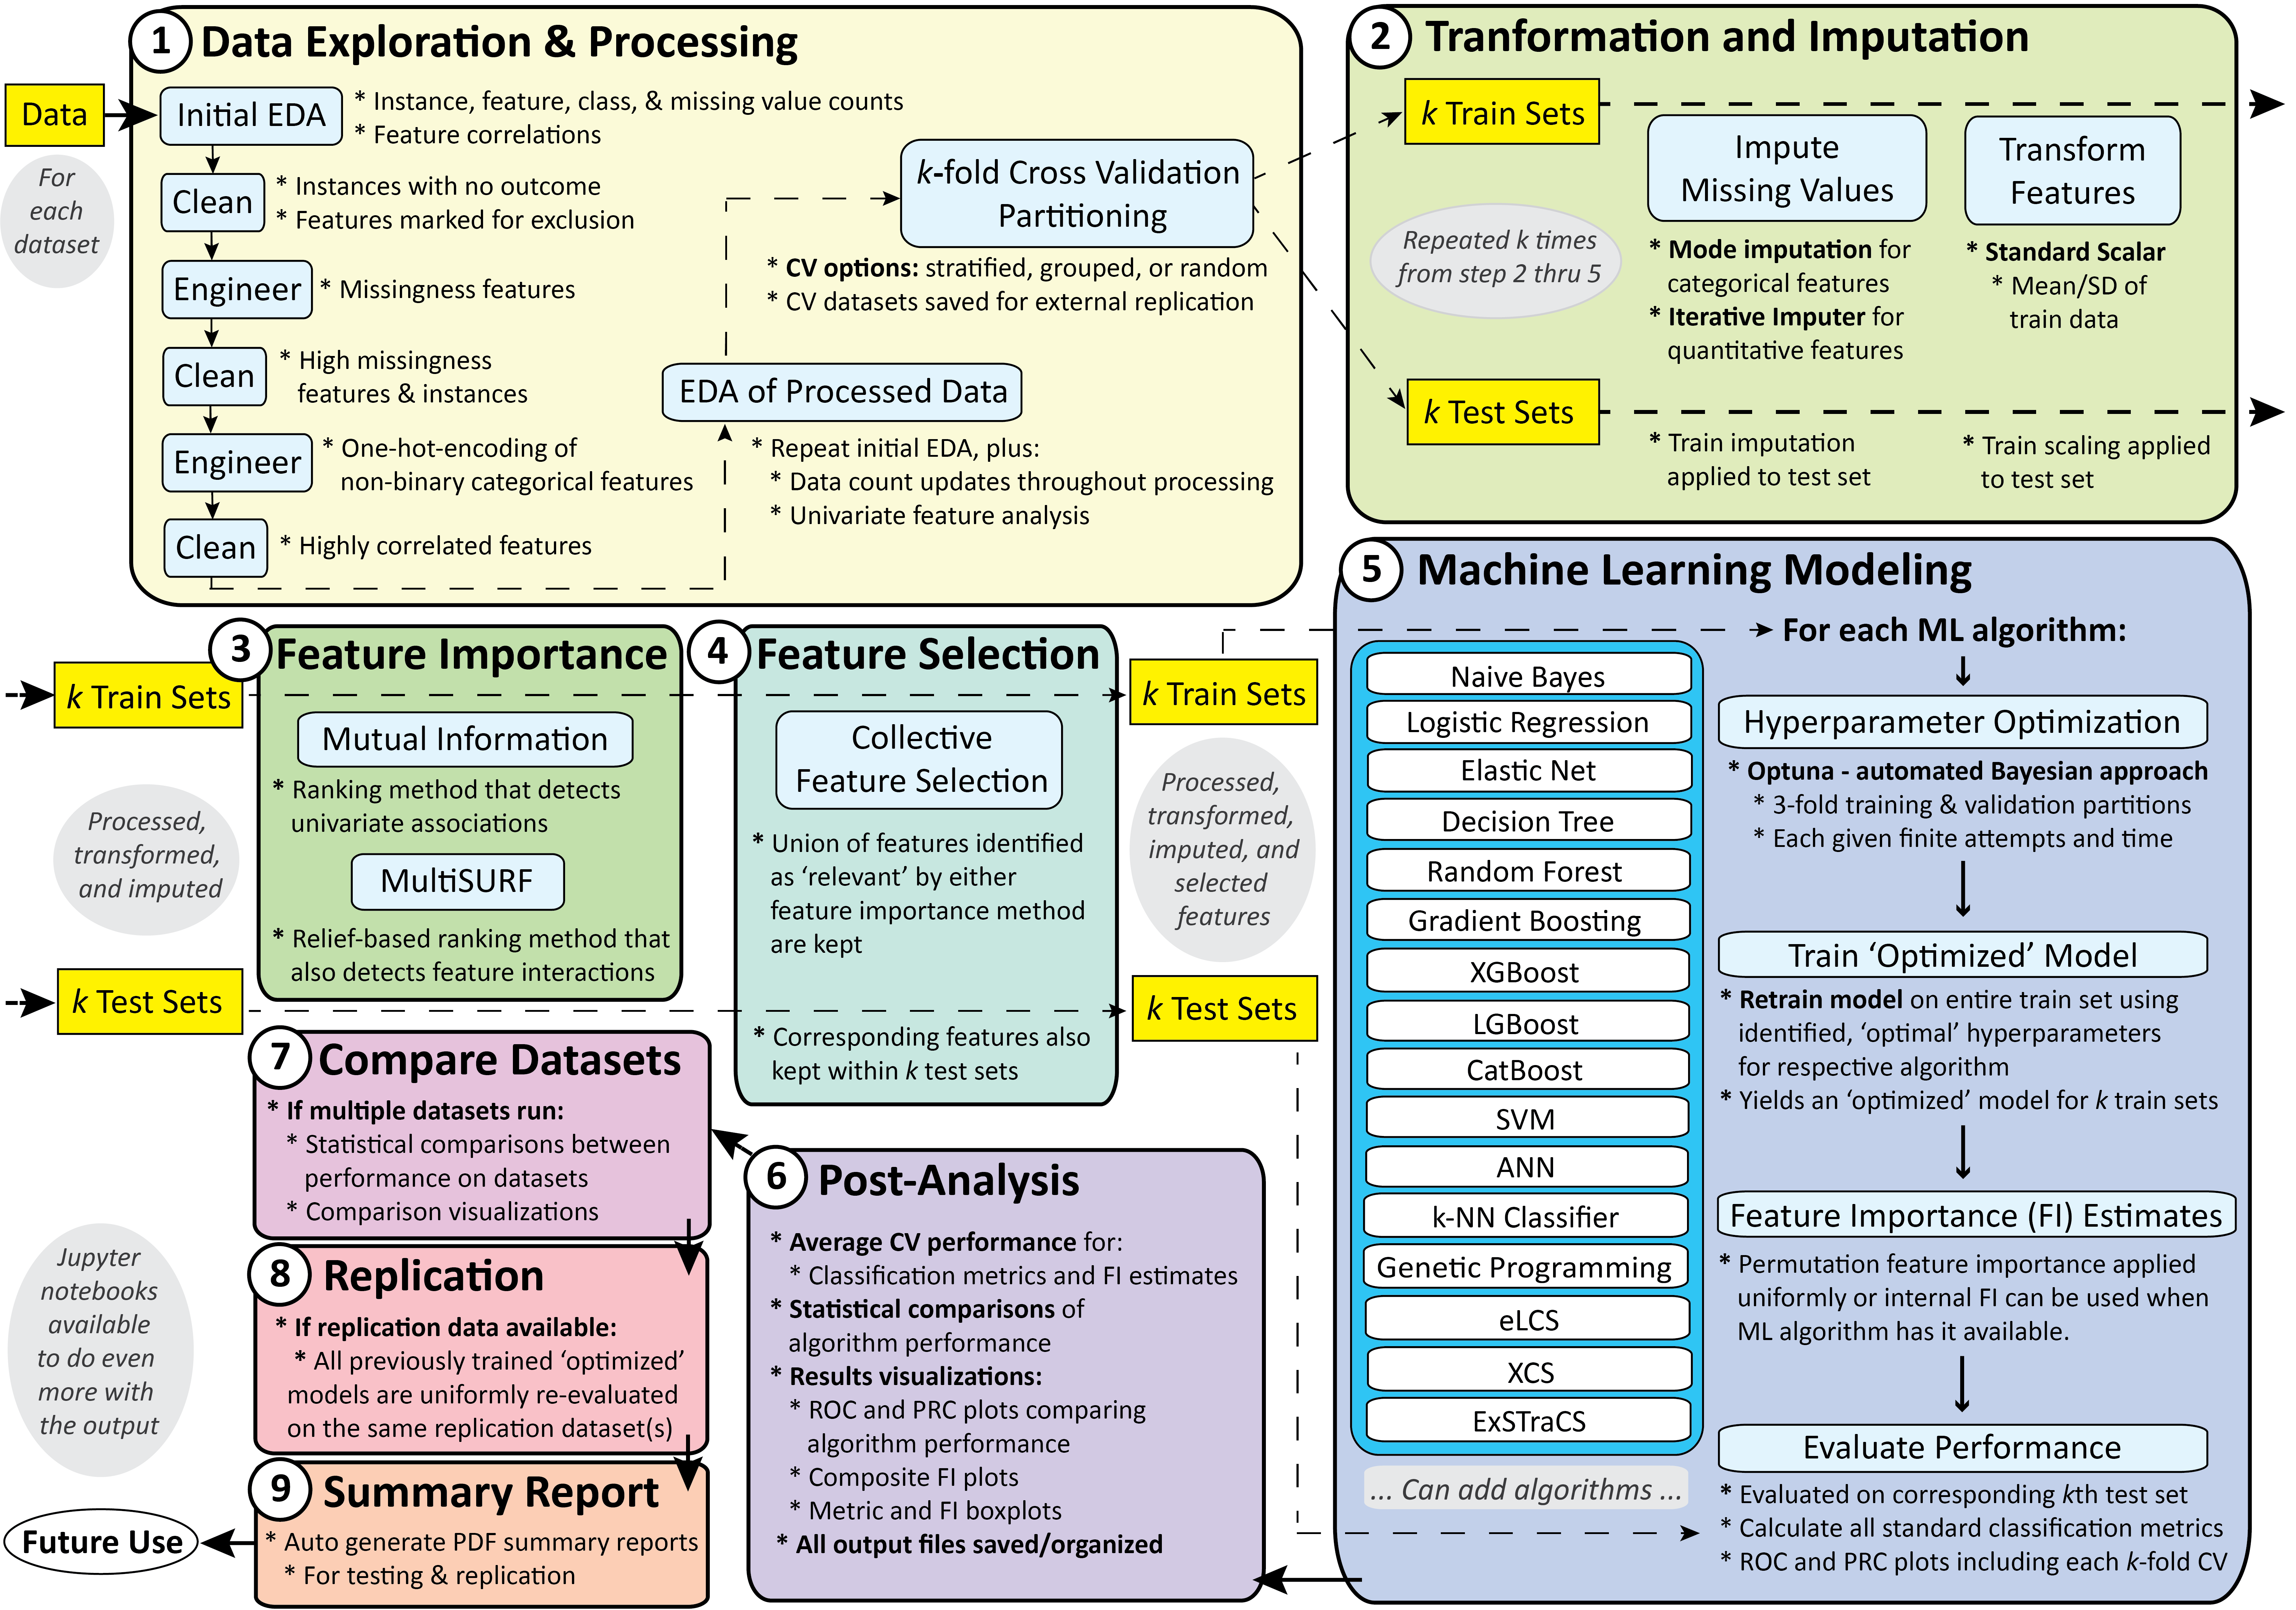
\includegraphics[width=1\textwidth]{figures/STREAMLINE_paper_lightcolor.png}
 \caption[Pipeline STREAMLINE]{\textbf{Schéma du pipeline STREAMLINE}. Ce pipeline est divisé en 4 parties principales: (i) traitement des données, (ii) calcul de l'importance et sélection des descripteurs, (iii) entrainnement et optimisation des modèles, (iv) post-traitement et comparaison des modèles. (\cite{urbanowicz_streamline_2023})}
 \label{fig:streamline}
\end{figure}
\subsection{Métriques de performance}
Pour évaluer les performances de nos modèles, nous avons utilisé plusieurs métriques. Dans le cadre d'une classification multi-classe et déséquilibrée, la mesure de l'exactitude de classification (\textit{accuracy}) n'est pas suffisante pour obtenir une bonne représentation des performances des modèles. Ainsi nous mesurons aussi l'exactitude équilibrée (\textit{balanced accuracy}), le score F1, score F1 macro, la spécificité et le coefficient de corrélation de Matthew. L'ensemble de ces métriques de performance, décrites dans la section suivante, sont calculées à partir de la matrice de confusion.

\subsubsection{Matrice de confusion}
La matrice de confusion est une matrice en deux dimensions qui compare  les prédictions d'un modèle par rapport aux labels réels des données. Par exemple pour une classification en 3 classes, une matrice de confusion de taille (3x3) est produite. La diagonale (haut gauche vers bas droit) représente l'ensemble des prédictions correctes (vrais positifs et vrais négatifs) c'est-à-dire les points pour lesquels la prédiction est en accord avec le label réel. Les autres cases représentent l'ensemble des prédictions incorrectes (faux positifs ou faux négatifs). La figure \ref{fig:confusion-example}  représente un exemple de matrice de confusion pour une classification binaire en 2 classes.
\begin{figure}[!ht]
 \centering
 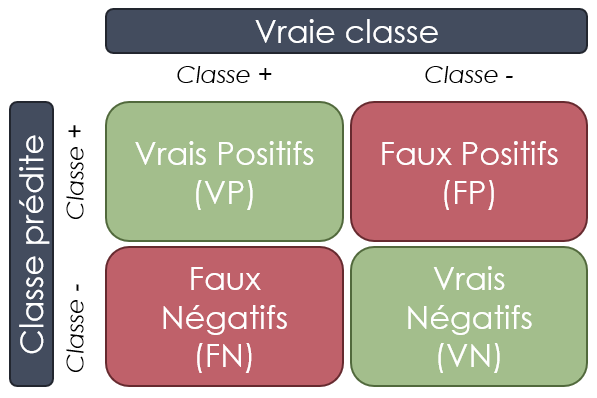
\includegraphics[width=0.5\textwidth]{figures/confusion_example.png}
 \caption[Exemple de matrice de confusion binaire]{Exemple de matrice de confusion binaire. Pour une classification à deux classes la matrices de confusion est composée de vraispositif (VP), vrais négatifs (VN), faux positifs (FP), faux négatifs (VN).}
 \label{fig:confusion-example}
\end{figure}

\subsubsection{Exactitude}
L'exactitude est une mesure de performance classique qui évalue la proportion de points de données correctement classées par rapport aux nombres totaux de points de données. Cette mesure est trompeuse dans le cadre de données déséquilibrées. Elle est calculée telle que :
\[ \text{Exactitude} = \frac{\text{Vrais Positifs} + \text{Vrais Négatifs}}{\text{Vrais Positifs} + \text{Vrais Négatifs} + \text{Faux Positifs} + \text{Faux Négatifs}} \]

\subsubsection{Exactitude équilibrée}
L'exactitude équilibrée quant à elle est utile dans le cadre d'un jeu de données déséquilibré. Elle donne une importance égale aux performances de chaque classe. Pour cela, l'exactitude (équivalente à la sensibilité dans un contexte multi-classe) est calculée pour chaque classe. Ensuite, l'exactitude équilibrée correspond donc à la moyenne de l'exactitude pour chaque classe. Ainsi sa formule est égale à :
\[ \text{Exactitude équilibrée} = \frac{1}{n} \sum_{i=1}^{n} \text{Exactitude}_i \] où \textit{n} représente le nombre de classes différentes.

\subsubsection{Précision, sensibilité, spécificité et Score F1}
La figure \ref{fig:prec_recall_spec} présente les notions de précision, sensibilité (rappel) et spécificité en prenant comme exemple l'interprétation d'un test COVID. Pour un test COVID, la précision représente la proportion de patients réellement positifs parmi des tests positifs. Le sensibilité (ou rappel) représente la proportion de tests positifs parmi l'ensemble des personnes positives à la COVID. Enfin la spécificité mesure la proportion de tests réellement négatifs parmi l'ensemble des patients négatifs au COVID.

\begin{figure}[!ht]
 \centering
 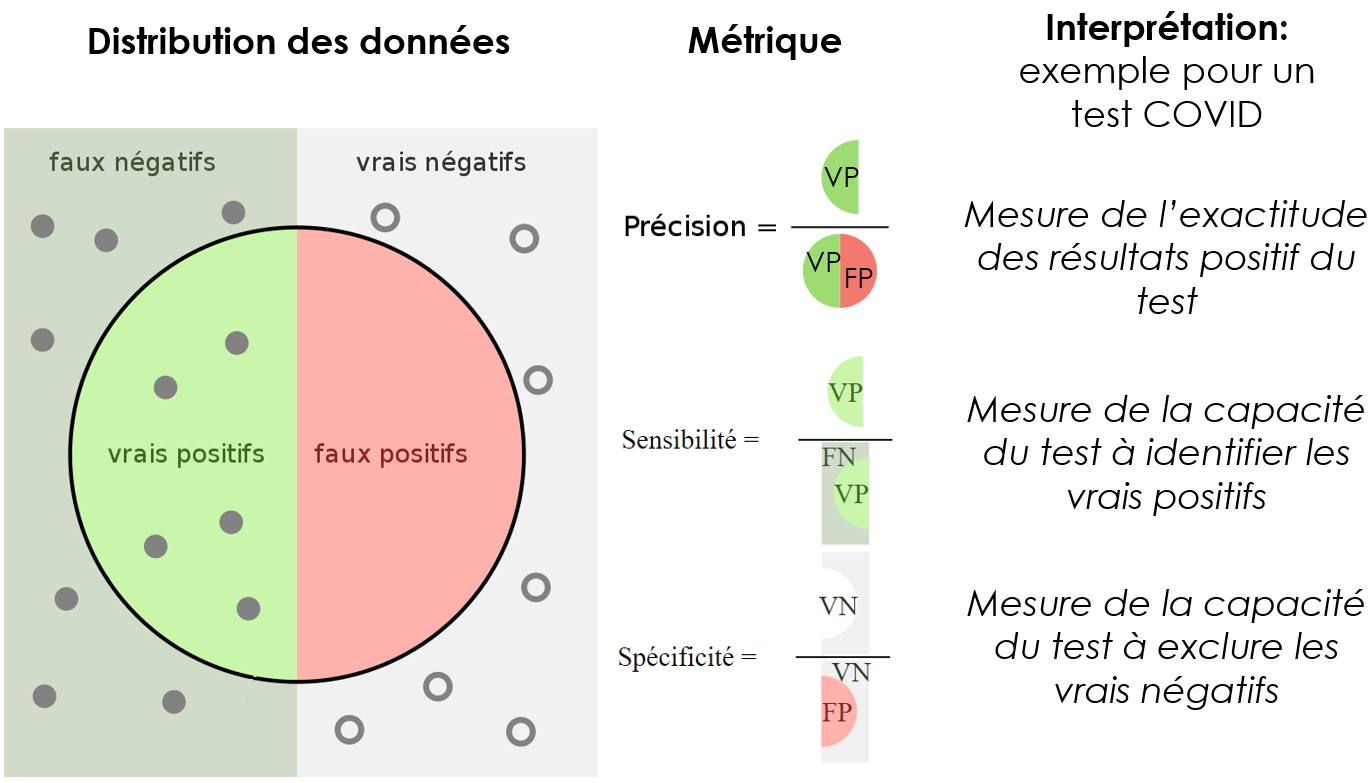
\includegraphics[width=1\textwidth]{figures/prec_recall.png}
 \caption[Précision, sensibilité et spécificité]{\textbf{Schéma de la notion de précision, sensibilité et spécificité} (modifié de Wikipédia "Précision et rappel").}
 \label{fig:prec_recall_spec}
\end{figure}

Le score-F1 correspond à la moyenne harmonique de la précision et de la sensibilité (rappel) et donc permet de tenir compte à la fois des faux positifs et des faux négatifs. Dans le cadre de classification multi-classe (3 et plus), le score F1 peut être calculé de plusieurs manières. Soit de manière "micro" c'est-à-dire globalement à partir du nombre de vrais positifs, faux négatifs et faux positifs. Soit de manière "macro", en calculant le score F1 de chaque classe et en réalisant leur moyenne, similairement à la différence entre exactitude et exactitude équilibrée. Ainsi la formule du score F1-Macro est :
\[ \text{Score F1 Macro} = \frac{1}{n} \sum_{i=1}^{n} \frac{2 \times \text{Précision}_i \times \text{Rappel}_i}{\text{Précision}_i + \text{Rappel}_i} \] où \(n\) représente le nombre de classes différentes.

\subsubsection{Coefficient de corrélation de Matthew}
Le \gls{mcc} est une métrique prenant en compte l'ensemble des éléments de la matrice de confusion (vrais positifs, faux positifs, vrais négatifs, faux négatifs), contrairement aux métriques présentées ci-dessus. De plus, elle est équilibrée, c'est-à-dire qu'elle n'est pas biaisée dans le cas de classes déséquilibrées. Ses valeurs sont comprises entre -1 et 1, avec 0 pour des prédictions aléatoires, 1 pour des prédictions parfaites et -1 pour des prédictions parfaitement contraires. Cette métrique est plus informative sur la qualité d'un modèle que le score F1 (\cite{chicco_advantages_2020}). Dans le cadre d'une classification binaire, la formule du MCC est :
\[ MCC = \frac{VP \times VN - FP \times FN}{\sqrt{(VP + FP)(VP + FN)(VN + FP)(VN + FN)}} \]
Dans le cadre d'une classification multi-classe, la formule est plus complexe :
\[ MCC = \frac{
    c \times s - \sum_{k}^{K} p_k \times t_k
}{\sqrt{
    (s^2 - \sum_{k}^{K} p_k^2) \times
    (s^2 - \sum_{k}^{K} t_k^2)
}} \]
où \(c\) représente le nombre d'échantillons correctement prédits, \(s\) représente le nombre total d'échantillons, \(p_k\) le nombre de fois où la classe k a été prédite, \(t_k\) le nombre de fois où la classe k s'est réellement produite.

\section{Techniques d'analyse d'image et réseaux de neurones}
Les méthodes que nous avons développées permettent d'analyser des données d'imagerie histologique. L'outil \gls{impatient} présenté dans le chapitre 5 permet de faire de l'annotation et segmentation d'image en utilisant des techniques d'analyse d'image traditionnelles. L'outil \gls{myoquant} présenté dans le chapitre 8 permet de faire de la quantification de marqueurs pathologiques grâce à la fois à des méthodes d'analyse traditionnelles, mais aussi grâce à des modèles préentrainés et des réseaux de neurones profonds.  Dans cette section nous allons voir les bibliothèques de codes, les modèles et le matériel que nous avons utilisés. 

\subsection{Méthodes d'analyse d'image traditionnelles avec scikit-image}
Pour l'analyse d'image en utilisant des méthodes traditionnelles nous avons utilisé la bibliothèque de code \textit{scikit-image} (\cite{walt_scikit-image_2014}, \url{https://scikit-image.org/}). \textit{Scikit-image} a été développé en 2014 et met à disposition des outils de base pour l'analyse d'image tel que le calcul de contraste, d'intensité et de texture de pixels qui sont des mesures utilisées par \gls{impatient} pour la segmentation d'image. Dans \gls{myoquant}, \textit{scikit-image} est utilisé pour tracer des lignes, réaliser de l'érosion d'image et mesurer des surfaces, périmètres, diamètre de Feret et la position des centroïdes à partir de masques de segmentation.

\subsection{Modèle préentrainé Cellpose et Stardist}
Dans le cadre de \gls{myoquant} nous avons utilisés des modèles préentrainés pour l'analyse des images de coupes histologiques. Pour la segmentation des fibres musculaires, nous avons utilisé l'implémentation Python du modèle Cellpose (\cite{stringer_cellpose_2021}, \url{https://github.com/MouseLand/cellpose}). Parmi les différents modèles inclus dans Cellpose, nous avons utilisé spécifiquement le modèle \textit{cyto2}, qui est le modèle disponible dans Cellpose le plus récent et performant pour la segmentation des fibres musculaires sous diverses colorations. 

Quant à la segmentation des noyaux cellulaires, nous avons utilisé l'implémentation Python du modèle Stardist (\cite{weigert_star-convex_2020}, \url{https://github.com/stardist/stardist}). Plus précisément dans le cadre de l'analyse des noyaux dans la coloration \gls{he}, nous avons utilisé le modèle préentrainé \textit{2D\_versatile\_he}, qui est un modèle spécifiquement entrainé sur des images à la coloration \gls{he}.

\subsection{Développement de réseaux de neurones profond de type ResNet avec Keras Tensorflow}
En plus des modèles préentrainés, dans \gls{myoquant} nous avons entrainé et intégré nos propres modèles de classification basés sur les réseaux de neurones profonds. Pour cela nous avons utilisé les bibliothèques de code Keras (\cite{chollet_keras_2015}, \url{https://keras.io/}) et Tensorflow (\cite{martin_abadi_tensorflow_2015}, \url{https://www.tensorflow.org/}). Keras est une bibliothèque qui permet une interaction simplifiée avec Tensorflow mettant à disposition plusieurs architectures de modèles préétablis ainsi que des fonctions permettant d'accélérer le développement de modèles de réseaux de neurones. Dans le cadre de développement de modèles de classification d'image, nous avons utilisé l'architecture RestNet50 version 2 préentrainée sur le jeu de données \textit{ImageNet} implémentée dans Keras. L'architecture ResNet50 (\cite{he_deep_2015}) est un réseau de neurones convolutifs composé de 48 couches convolutives. Ce modèle possède un total de 23 564 800 paramètres. L'entrainement de ce modèle et son inférence sur des données d'imagerie ont été réalisés sur des machines virtuelles de la plateforme SCIGNE Grand-Est équipée de \gls{gpu} RTX 2080 Ti.

\section{Développement d'outils basés sur modèles linguistiques de grande taille}
Les méthodes que nous avons développées (\gls{nlmyo}) pour analyser du texte libre (compte rendu de biopsie) se basent sur les modèles linguistiques de grande taille. Dans cette section, nous détaillons les outils et modèles que nous avons utilisés.

\subsection{Reconnaissance de texte avec Tesseract}
Dans un premier temps, comme la majorité des comptes rendus sont au format PDF il est nécessaire de les convertir en texte. Pour cela, nous avons utilisé des méthodes d'\gls{ocr}. L'outil libre que nous avons utilisé pour cela se nomme Tesseract (\cite{ray_tesseract_2015}) version 5, mise à disposition en novembre 2021. Cet outil est capable de reconnaitre de manière robuste du texte dactylographié dans plus de 100 langues différentes.

\subsection{Modèles linguistiques de grande taille utilisés}
Dans le cadre du développement de \gls{nlmyo} nous avons utilisé 2 \gls{llms} génératifs et 2 \gls{llms} d'embedding. Pour chaque catégorie de \gls{llms} nous avons voulu comparer les résultats issus de modèles provenant de fournisseurs externes (OpenAI) par rapport à des modèles plus petits hébergés localement.

\subsubsection{Modèles génératifs : OpenAI GPT-3.5 et Vicuna-7B}
Un des critères déterminants pour le choix de modèle génératif est les performances du modèle et la taille de contexte. La taille de contexte pour un \gls{llms} représente le nombre de mots qu'il est capable de traiter lors d'une requête. Ainsi plus la taille de contexte est grande, plus il est possible d'analyser un document de grande taille avec des instructions détaillées. Par exemple, le modèle GPT-3.5-turbo d'OpenAI a une taille de contexte de 4096 jetons, ce qui représente environ 3000 mots en anglais. 

La grande majorité des modèles open source et auto-hébergeable ont une taille de contexte de 512, ce qui limite leur utilisation pour l'analyse de grands documents. Notre choix de modèle autohébergeable s'est porté sur le modèle Vicuna-7B-1.1 (\cite{chiang_vicuna_2023}, \url{https://huggingface.co/vicuna/ggml-vicuna-7b-1.1}), qui en plus d'être un modèle de petite taille (7 milliards de paramètres par rapport aux 175 milliards de paramètres de GPT-3.5-turbo) donc requérant de faible ressources informatiques, possède une taille de contexte de 2048. De plus ce modèle est actuellement le plus  performant parmi les modèles open source de taille 7B (\cite{hendrycks_measuring_2021}). 

Concernant le modèle provenant d'un fournisseur externe, nous avons choisi d'utiliser GPT-3.5-turbo d'OpenAI, car ce modèle allie à la fois une  grande taille de contexte de 4096, d'excellentes performances (4e modèle le plus performant toutes catégories confondues \cite{lianmin_zheng_chatbot_2023}) et possède une \gls{api} accessible à bas coût (0,002 \$ par tranche de 1000 \textit{tokens}).

Pour finir, pour les deux modèles génératifs, nous avons mis le paramètre de température le plus proche de 0 possible, c'est-à-dire à 0,01. Le paramètre de température contrôle le niveau de hasard des réponses du modèle. Plus ce paramètre est proche de 0, plus la réponse du modèle est déterministe. Plus cette valeur est supérieure à 1, plus la sortie est aléatoire. La valeur par défaut du modèle est 1. Ainsi en mettant ce paramètre très proche de 0, les résultats sont reproductibles. 

\subsubsection{Modèle d'\textit{embedding} : OpenAI et Instructor}
Les \gls{llms} d'embedding sont des modèles qui transforment du texte en vecteur numérique, ce qui permet de faire de la classification, du clustering et de la recherche de similarité. Ces modèles sont utilisés dans \gls{nlmyo} pour faire de la prédiction de diagnostic et pour créer un moteur de recherche de patients.

Comme pour les modèles  génératifs, nous avons utilisé deux modèles, un par un fournisseur externe et un autohébergé pour comparer les performances. En termes de choix de modèles, pour le modèle issu de fournisseurs externes, nous avons utilisé le modèle d'\textit{embedding} nommé text-embedding-ada-002, car nous utilisons déjà le modèle génératif du même fournisseur (OpenAI). De plus ce modèle est multilangue et performant, car il est classé 6e en termes de performances d'\textit{embedding} sur 75 modèles testés à travers un panel de 56 jeux de données (\cite{muennighoff_mteb_2022}).

Concernant le modèle autohébergé, nous avons choisi d'utiliser le modèle nommé Instructor (\cite{su_one_2023}, \url{https://huggingface.co/hkunlp/instructor-large}). Ce modèle est parmi les plus performants, classé 2e sur 75 modèles testés (\cite{muennighoff_mteb_2022}), de plus il comporte dans son jeu d'entrainement des données issues de textes médicaux, ce qui permet d'espérer de bonnes performances pour nos comptes rendus de biopsies. 

\subsection{Interaction avec les modèles linguistiques de grande taille avec LangChain}

Face à la diversité des \gls{llms} génératifs, \gls{llms} d'\textit{embedding} et des outils associés, il est nécessaire d'avoir un outil qui uniformise la façon d'interagir avec ces modèles. C'est l'objectif de la bibliothèque de code nommée LangChain (\cite{chase_harrison_langchain_2022}) que nous avons utilisé à travers \gls{nlmyo}. Cette bibliothèque de code permet d'unifier la façon d'interagir avec les modèles autohébergés et les différents fournisseurs externes, ce qui permet d'accélérer la phase d'exploration des performances des modèles et le développement d'outils basés sur les \gls{llms}. 

En plus des interactions avec les modèles de langage, LangChain met à disposition des outils pour interagir avec des bases de données optimisées pour le stockage et la requête de vecteurs numériques (résultats des modèles d'\textit{embedding}). Ainsi dans \gls{nlmyo} nous avons utilisé la base de données de vecteurs nommée ChromaDB (\url{https://www.trychroma.com/}). Les bases de données de vecteurs sont des bases de données qui permettent de stocker des documents ainsi que leurs résultats d'\textit{embedding}. Ces bases sont optimisées pour le calcul de similarité entre un vecteur requête et une grande base de données de vecteurs. Cela permet par exemple de construire des moteurs de recherche de documents, dans notre cas il s'agit d'un moteur de recherche de comptes rendus de biopsie requêtables par symptômes.

\section{Développement d'outils et d'interfaces}
Les divers outils que nous avons développés dans cette thèse (\gls{impatient}, \gls{nlmyo}, \gls{myoquant}) sont disponibles sous différentes formes : applications web complètes, démonstrations en ligne, outils en ligne de commande.  Pour cela, nous avons utilisé diverses bibliothèques de code spécifique à chaque cas de figure.

\subsection{Développement d'une application web complète pour IMPatienT}
Dans le cadre du développement de notre application web et base de données \gls{impatient} nous avons entièrement construit une application web. Les applications web sont composées de trois éléments : l'interface (nommée \textit{front-end}), le serveur de calcul (nommé \textit{back-end}) et la base de données. Pour construire l'interface de \gls{impatient}, nous avons utilisé la bibliothèque de code graphique CSS BootStrap 5 (\cite{mark_otto_bootstrap_2011}) couplée à la bibliothèque de code JavaScript JQuery 3.7 (\cite{resig_jquery_2006}) pour l'interactivité du site. Concernant la partie serveur, nous avons utilisé la bibliothèque de code Python nommée Flask (\cite{ronacher_flask_2010}).  Nous avons utilisé Flask car c'est une bibliothèque minimale et bien documentée qui permet de construire un site web rapidement en augmentant graduellement la complexité. Enfin, en guise de base de données, nous avons utilisé le système de base de données relationnelle SQLite \cite{hipp_sqlite_2020}. Le système SQLite a l'avantage d'être léger et portable, car la base de données n'est composée que d'un seul fichier tout en proposant presque les mêmes fonctionnalités que les systèmes de base de données relationnelles plus complexes.

\subsection{Développement d'un outil en ligne de commande pour MyoQuant}
Dans le cadre du développement de notre outil d'analyse d'images \gls{myoquant}, nous avons décidé de rendre l'outil disponible d'abord sous la forme d'outil en ligne de commande. En effet, comme \gls{myoquant} est voué à analyser des images de grande taille pendant des temps d'analyse longs et sur des ordinateurs avec de l'équipement spécialisé, l'outil en ligne de commande semble être la modalité la plus adaptée. Pour cela nous avons utilisé les bibliothèques de code python nommées Typer (\cite{ramirez_typer_2019}) et Rich (\cite{will_mcgugan_rich_2020}). Typer permet de créer des commandes complexes pour un outil en ligne de commande, de valider les paramètres et de générer automatiquement la documentation nécessaire à l'outil, tandis que Rich permet d'enrichir l'expérience de l'usage de la ligne de commande en affichant des données formatées directement dans le terminal (en couleur, sous forme de tableau, interactives etc.).

\subsection{Développement de démonstrations en ligne pour NLMyo et MyoQuant}
Enfin, pour le développement de \gls{nlmyo} mais aussi pour \gls{myoquant} nous avons voulu développer des applications de démonstration en ligne. Ces applications de démonstration ont pour but de faciliter la communication autour des outils et de pouvoir démontrer leur utilité. Pour cela nous avons utilisé la bibliothèque de code Python nommée Streamlit (\cite{adrien_treuille_streamlit_2018}). Streamlit permet de construire des applications web simples et interactives très rapidement sans avoir à gérer la partie interface et serveur séparément, le tout dans un seul et même langage de programmation. L'utilisation de Streamlit nous a permis de mettre en place, de modifier et d'affiner rapidement des démonstrations de nos outils basés sur l'IA.

\section{Recherche ouverte et reproductibilité}
La recherche ouverte est essentielle, notamment en \gls{ia} pour faciliter l'adoption des outils, les améliorer et permettre leur analyse critique. Dans cette optique de science ouverte, nous avons utilisé différents outils pour partager nos travaux de recherche de façon libre et ouverte et les rendre reproductibles.

\subsection{Développement open source et versionnage avec GitHub}
Le code correspondant à l'ensemble des outils et des travaux présentés dans cette thèse est disponible de façon libre et open source sur mon profil GitHub (\url{https://github.com/lambda-science}). GitHub est une société fondée en 2008 qui permet le versionnage de code informatique. Le versionnage est un système qui permet de traquer les modifications apportées  au code dans le temps et de garder une trace de toutes les versions qui ont existé. L'utilisation de tels systèmes facilite la collaboration en permettant à n'importe qui de contribuer au code, de proposer des améliorations ou de signaler des problèmes éventuels.

\subsection{Développement de données et modèles IA open source avec HuggingFace}
Si GitHub permet de versionner le code, il est aussi nécessaire d'avoir des outils permettant de rendre public et versionnable les modèles d'\gls{ia} entrainés et les données utilisées. Mettre à disposition les modèles IA et les données utilisées de façon open source permet à la communauté d'évaluer de manière indépendante les modèles, mais aussi de les améliorer en entrainant de meilleurs à partir du jeu de données de base. Pour cela, nous avons mis en ligne les données utilisées pour entrainer le modèle SDH de \gls{myoquant} ainsi que le modèle avec son code d'entrainement sur la plateforme HuggingFace à l'adresse : \url{https://huggingface.co/corentinm7}. HuggingFace est une société fondée en 2016 qui permet de mettre en libre accès des jeux de données et des modèles d'\gls{ia} de manière open source. De plus, HuggingFace développe de nombreuses bibliothèques de code Python open source spécialisées en \gls{ia} comme la bibliothèque nommée \textit{transformers} qui permet l'entrainement de \gls{llms}.

\subsection{Suivi d'expérience avec \textit{Weight and Biais}}
L'entrainement d'un modèle \gls{ia} est un processus long qui passe par de nombreuses phases de recherche sur les algorithmes et les architectures les plus performantes, les paramètres optimaux ou le meilleur prétraitement des données pour obtenir  un modèle performant. Pour traquer les performances des divers modèles entrainés et les comparer, des outils existent à l'instar de GitHub et HuggingFace. Dans cette thèse j'ai utilisé l'outil nommé \textit{Weight and Bias} (\url{https://wandb.ai/}), une société fondée en 2017, pour traquer les performances des divers entrainements des modèles de \gls{myoquant} et \gls{nlmyo}. Dans les chapitres suivants, un lien vers les résultats en ligne est fourni pour accéder à l'ensemble des informations enregistrées.

\subsection{Environnement de développement reproductible}
Le dernier élément concernant la reproductibilité des travaux après avoir fourni le code, les données et les modèles de manière open source reste de s'assurer que le code puisse s'exécuter correctement quel que soit l'environnement informatique. Pour cela, pour chaque outil, nous fournissons deux éléments. En premier nous fournissons un environnement virtuel Python avec Poetry (\url{https://python-poetry.org/}) qui permet de spécifier les versions exactes de bibliothèques de code python utilisées ainsi que les versions de leurs dépendances. De plus, nous construisons une image Docker (\url{https://www.docker.com/}) pour chaque outil ce qui permet non seulement de contrôler la version de Python utilisée, mais aussi le système d'exploitation et les versions de ses diverses bibliothèques de codes annexes. L'utilisation d'images Docker couplée à un environnement virtuel Python spécifique permettent de s'assurer que notre code fonctionne et est reproductible sur n'importe quel matériel informatique.

\subsection{Archivage du code, des données et des résultats avec Zenodo}
Zenodo  (\cite{european_organization_for_nuclear_research_zenodo_2013}, \url{https://zenodo.org/}) est un outil développé par le \gls{cern} en 2013, qui permet d'archiver des travaux de recherche, du code et des données et d'y associer un identifiant unique citable (\gls{doi}). Dans le cadre de cette thèse, nous avons créé une archive Zenodo qui contient l'ensemble des éléments de cette thèse, c'est-à-dire : le manuscrit, le code des outils, les données non confidentielles utilisées, les modèles entrainés et les figures et les résultats. Le lien vers cette archive est \url{https://doi.org/10.5281/zenodo.8163664}.